\documentclass[a5paper,10pt]{article}
\newcommand{\MyTitle}{De tillresta - Spelarbok}
\documentclass[a5paper,10pt]{article}

\usepackage[utf8]{inputenc}
\usepackage[swedish]{babel}
\usepackage[T1]{fontenc}
\usepackage[pdftex]{graphicx}
\usepackage{calc,xparse,geometry}
\usepackage{wrapfig}
\usepackage[pagestyles]{titlesec}

\graphicspath{ {./../Bilder/} }
\newpagestyle{mine}{%
\sethead[\thepage][{\raisebox{\dimexpr\headheight + \topmargin + \voffset + 1in-0.75in\relax}[0pt][0pt]{
\includegraphics[width = .75\textwidth]{horn}}}][]
{}{{\raisebox{\dimexpr\headheight + \topmargin + \voffset + 1in-0.75in\relax}[0pt][0pt]{
\includegraphics[width = .75\textwidth]{horn}}}}{\thepage}
\setfoot{}{}{}
}
\pagestyle{mine}
\author{Gustav Ruthgård}
\title{\MyTitle}
\date{\today}

\usepackage{xkeyval}

\makeatletter
\define@cmdkey{rpg}[char@]{name}[]{}
\define@cmdkey{rpg}[char@]{class}[]{}
\define@cmdkey{rpg}[char@]{kropp}[]{}
\define@cmdkey{rpg}[char@]{reaktion}[]{}
\define@cmdkey{rpg}[char@]{sinne}[]{}
\define@cmdkey{rpg}[char@]{special}[]{}
\define@cmdkey{rpg}[char@]{width}[\linewidth]{}

\define@cmdkey{move}[char@]{rubrik}[]{}
\define@cmdkey{move}[char@]{beskrivning}[]{}
\define@cmdkey{move}[char@]{grundegenskap}[]{}
\define@cmdkey{move}[char@]{lyckat}[]{}
\define@cmdkey{move}[char@]{mitten}[]{}
\define@cmdkey{move}[char@]{misslyckat}[]{}
\define@cmdkey{move}[char@]{val}[]{}
\define@cmdkey{move}[char@]{width}[\linewidth]{}

\define@cmdkey{scenen}[char@]{typ}[]{}
\define@cmdkey{scenen}[char@]{namn}[]{}
\define@cmdkey{scenen}[char@]{rubrik}[]{}
\define@cmdkey{scenen}[char@]{plats}[]{}
\define@cmdkey{scenen}[char@]{birollett}[]{}
\define@cmdkey{scenen}[char@]{birolltva}[]{}
\define@cmdkey{scenen}[char@]{birolltre}[]{}
\define@cmdkey{scenen}[char@]{width}[\linewidth]{}

\newcommand{\statlabel}{\textsc}

\usepackage{calc,xparse}
\newlength\mycardwidth
\setlength\mycardwidth{.75\textwidth}
\NewDocumentCommand \boxme { O{} }{%
  \fbox{%
    \parbox{\linewidth-2\fboxrule-2.5\fboxsep}{\strut #1}%
  }%
}
\NewDocumentCommand \pageme { O{} O{} }{%
  \begin{minipage}{#1\mycardwidth}
    \centering\boxme[#2]
  \end{minipage}%
}
\NewDocumentCommand \cardme { O{.75\textwidth} +m }{%
  \setlength\mycardwidth{#1-2\fboxrule-2\fboxsep}%
  \fbox{%
    \begin{minipage}{\mycardwidth}
      \centering
      #2%
    \end{minipage}%
  }%
}

\newcommand{\setcharacterstats}[1]{%
  \begingroup
  \setkeys{rpg}{name,class,kropp,reaktion,sinne,special,width,#1}%
  \noindent
  \cardme[\textwidth]{%
    \pageme[.69][\statlabel{Namn}: \char@name]%
    \pageme[.31][\statlabel{\char@class}]

    \pageme[.33][\statlabel{Kropp}: \char@kropp]%
    \pageme[.34][\statlabel{Reaktion}: \char@reaktion]%
    \pageme[.33][\statlabel{Sinne}: \char@sinne]
    \raggedright \textit{S�tt ut +2, +1, 0}

    \pageme[][\statlabel{Specialdrag}:]
    \raggedright \textit{\char@special}
  }
}
\newcommand{\displaymove}[1]{%
  \begingroup
  \setkeys{move}{rubrik,beskrivning,grundegenskap,lyckat,mitten,misslyckat,val,width,#1}%
  \noindent
  \cardme[\textwidth]{%
    \pageme[.69][\statlabel{\char@rubrik}]%
    \pageme[.31][\statlabel{Sl�} +\char@grundegenskap]

    \pageme[.99][\char@beskrivning]

    \pageme[.31][\statlabel{10+}]%
    \pageme[.69][\char@lyckat]

    \pageme[.31][\statlabel{7-9}]%
    \pageme[.69][\char@mitten]

    \pageme[.31][\statlabel{2-6}]%
    \pageme[.69][\char@misslyckat]

    \pageme[.99][\char@val]%
  }
}
\newcommand{\satscen}[1]{%
  \begingroup
  \setkeys{scenen}{typ,namn,rubrik,plats,birollett,birolltva,birolltre,width,#1}%
  \noindent
  \cardme[\textwidth]{%
    \pageme[1][\statlabel{\textbf{\char@typ}}]

    \pageme[1][\statlabel{Rubrik:} \char@rubrik]

    \pageme[.31][\statlabel{Huvudroll:} \char@namn]%
    \pageme[.69][\statlabel{Plats:} \char@plats]

    \pageme[1][\statlabel{Plats:} \char@plats]

    \pageme[.33][\statlabel{Biroll: } \char@birollett]%
    \pageme[.34][\statlabel{Biroll: } \char@birolltva]%
    \pageme[.33][\statlabel{Biroll: } \char@birolltre]
  }
}
\newcommand{\rollformular}[1]{%
  \begingroup
  \setkeys{rpg}{name,class,kropp,reaktion,sinne,special,width,#1}%
  \noindent
  \cardme[\textwidth]{%
    \pageme[.69][\statlabel{Namn}: \char@name]%
    \pageme[.31][\statlabel{Koncept}:]
    \pageme[][\statlabel{R�dsla}:]
    \pageme[][\statlabel{Drivkraft}:]

    \pageme[.33][\statlabel{Kropp}: \char@kropp]%
    \pageme[.34][\statlabel{Reaktion}: \char@reaktion]%
    \pageme[.33][\statlabel{Sinne}: \char@sinne]
    \pageme[][\statlabel{Specialdrag}:]
  }
}
\makeatletter

\begin{document}
\maketitle
\clearpage
\section{Introduktion}
Det här rollspelets regler baseras på idéer ur Apocalypse World och kan därför räknas som ett så kallat PbtA spel, eller Powered by the Apocalypse spel. Spelardragen är inspirerade av Kult: Divinity Losts spelardrag.

Alla spelare kommer ha karaktärer som är födda i den lilla orten Marylain som ligger 6 mil väster om New Orleans i den amerikanska södern. Din karaktär är född 1977 och har någon gång mellan 1995 och 1999 flyttat ifrån Marylain för jobb eller högre studier.
\section{Koncept}
Ditt koncept är grundinriktningen för din rollperson, det definierar vilken typ av karaktär den du spelar har, det ger också en känsla för vilken bakgrund karaktären har. Följande koncept finns att välja bland:
\begin{itemize}
  \item Agenten
  \item Korren
  \item Atleten
  \item Familjevårdaren
  \item Politikern
  \item Förbrytaren
\end{itemize}
\subsection{Grundegenskaper}
I det här rollspelet finns tre grundegenskaper. När du slår för ett spelardrag använder du två sexsidiga tärningar och lägger ihop resultatet med grundegenskapen.
\begin{itemize}
  \item \statlabel{Kropp} beskriver din fysiska förmåga i spelet. Både styrka och smidighet ryms inom begreppet kropp. Följande drag baseras på kropp.
  \begin{itemize}
    \item Din förmåga att attackera.
    \item Din förmåga att undvika fysiska utfall
    \item Din förmåga att uthärda fysisk skada.
  \end{itemize}
  \item \statlabel{Reaktion} beskriver din förmåga att uppfatta vad som händer runt din rollperson. Följande drag baseras på reaktion.
  \begin{itemize}
    \item Din förmåga att överblicka en situation.
    \item Din förmåga att läsa av en person.
  \end{itemize}
  \item \statlabel{Sinne} beskriver hur vässat din rollpersons sinne är. Följande drag baseras på sinne.
  \begin{itemize}
    \item Din förmåga att efterforska information eller att undersöka en plats.
    \item Din förmåga att övertala andra på olika sätt.
    \item Din förmåga att behålla kontrollen.
  \end{itemize}
\end{itemize}
\subsection{Rädsla och drivkraft}
Din rädsla och din drivkraft definierar din karaktär på ett viktigt sätt och hjälper dig att ta beslut utifrån din karaktärs perspektiv istället för ditt eget.
Du väljer ett av varje i listan på det koncept du valt eller väljer ett eget i samråd med spelledaren.
\subsection{Att bli bättre}
Varje gång du misslyckas helt med ett drag och får 6 eller lägre så noterar du en erfarenhetspoäng, man lär sig av sina misstag. Efter varje spelmöte delas också erfarenhetspoäng enligt listan:
\begin{itemize}
  \item Har du lärt dig något nytt om världen? Ta 1 erfarenhetspoäng.
  \item Har du ensam eller tillsammans med gruppen löst ett större problem? Ta 2 erfarenhetspoäng.
  \item Har någon annan gjort något som bidragit till ett bra spelmöte? Ge en erfarenhetspoäng till den.
\end{itemize}
Du kan använda dina erfarenhetspoäng enligt tabellen nedan.
\begin{table}[!h]
  \begin{tabular}{|c|c|}
  \hline Du lär dig ett extra specialdrag & 7xp \\
  \hline Du ökar en av dina grundegenskaper & 10xp \\
  \hline
  \end{tabular}
\end{table}
\clearpage
\part{Koncept}
\section{Agenten}
\textit{Du arbetar som någon form av rättvisans beskyddare, det kan till exempel vara en polis, utredare, detektiv, eller hemlig polis. Att ordningen i samhället upprätthålls är ditt ansvar. Jobbet är på obekväma tider och du förväntas kunna ställa upp när som helst.}
\vskip1em
\setcharacterstats{
  class = Agent,
  special = Välj 1 av Skytt Detektiv eller Förhörsteknik
  }
\subsection{Specialdrag}
Välj ett specialdrag för din karaktär.
\subsubsection{Skytt}
\textit{När du agerar i strid med ett skjutvapen}, agerar du med +2 i modifikation.
\subsubsection{Detektiv}
\textit{När du undersöker något brottsrelaterat}, agerar du med +2 i modifikation.
\subsubsection{Förhörsteknik}
\textit{När du förhör någon}, agerar du med +2 i modifikation.
\subsection{Rädsla}
Välj en rädsla eller hitta på en egen till din karaktär.
\begin{itemize}
  \item Att förlora jobbet.
  \item Att inte kunna skydda dina vänner.
  \item Att något ur din bakgrund blir uppdagat av dina vänner.
\end{itemize}
\subsection{Drivkraft}
Välj en drivkraft eller hitta på en egen till din karaktär.
\begin{itemize}
  \item Lagen dömmer alla lika.
  \item Med lagen som förtecken finner jag makt.
  \item Jag är här för att hjälpa de svaga.
\end{itemize}
\clearpage
\section{Korren}
\textit{Du arbetar med någon form av journalistiskt yrke, det kan till exempel vara en tidningsreporter, redaktör, korrespondent, vloggare eller grävande journalist. Att allmänheten får reda på vad som händer i samhället är ditt ansvar.}
\vskip1em
\setcharacterstats{
  class = Korre,
  special = Välj 1 av Informationssökning Intervjuvteknik eller Press
  }
\subsection{Specialdrag}
Välj ett specialdrag för din karaktär.
\subsubsection{Informationssökning}
\textit{När du söker information}, agerar du med +2 i modifikation.
\subsubsection{Intervjuvteknik}
\textit{När du frågar ut någon}, agerar du med +2 i modifikation.
\subsubsection{Press}
\textit{När du agerar under hot på allmän plats}, agerar du med +2 i modifikation om du kan yrka på att du är Press.
\subsection{Rädsla}
Välj en rädsla eller hitta på en egen till din karaktär.
\begin{itemize}
  \item Att bli skadad av de som hotar dig.
  \item Att ditt material inte skall publiceras.
  \item Att inte ha råd att betala hyran.
\end{itemize}
\subsection{Drivkraft}
Välj en drivkraft eller hitta på en egen till din karaktär.
\begin{itemize}
  \item Sanningen måste fram.
  \item Allas påståenden måste ifrågasättas.
  \item Det finns mer som döljer sig i världen än vad folk tror.
\end{itemize}
\clearpage
\section{Atleten}
\textit{Du arbetar med någon form av atletiskt yrke, det kan till exempel vara en elitidrottare, gymnastiklärare, eller fysioterapeft. Att hålla din kropp i sjukt god kondition och även att motivera andra till det samma är din vardag.}
\vskip1em
\setcharacterstats{
  class = Atlet,
  special = Välj 1 av Närstrid Taktiker eller Lagspelare
  }
\subsection{Specialdrag}
Välj ett specialdrag för din karaktär.
\subsubsection{Närstrid}
\textit{När du agerar i en strid och din kroppsliga fysik är avgörande}, agerar du med +2 i modifikation.
\subsubsection{Taktiker}
\textit{När du agerar i en situation där praktisk taktik avgör utgången}, agerar du med +2 i modifikation.
\subsubsection{Lagspelare}
\textit{När du hjälper eller hindrar någon annan att agera i en farlig eller taktisk situation}, agerar du med +2 i modifikation.
\subsection{Rädsla}
Välj en rädsla eller hitta på en egen till din karaktär.
\begin{itemize}
  \item Att bli så skadad att du inte kan fortsätta tävla.
  \item Att bli utnyttjad igen.
  \item Att skada någon annan på riktigt.
\end{itemize}
\subsection{Drivkraft}
Välj en drivkraft eller hitta på en egen till din karaktär.
\begin{itemize}
  \item Att ständigt utmana din egen förmåga.
  \item Att stå i centrum och få allas beundran.
  \item Att visa för din far/mor att du duger.
\end{itemize}
\clearpage
\section{Familjevårdaren}
\textit{Du är den som tar hand om hemmet, familjen och din partner. Du är hemmaman eller hemmafru och är extremt bra på det. Att familjen fungerar väl, har en fungerande social kontakt med de andra i vänkretsen och att hemmet är i toppskick med skinande ytor och toppiffade fönsterbrädor är din förtjänst.}
\vskip1em
\setcharacterstats{
  class = Familjevårdare,
  special = Välj 1 av Minglaren Silvertunga eller Behärskad
  }
\subsection{Specialdrag}
Välj ett specialdrag för din karaktär.
\subsubsection{Minglaren}
\textit{När du småpratar med någon så får du alltid reda på något intressant}, agerar du med +2 i modifikation för att läsa av en person.
\subsubsection{Silvertunga}
\textit{När du försöker få din vilja igenom}, agerar du med +2 i modifikation när du försöker övertala en person.
\subsubsection{Behärskad}
\textit{Du har en mycket fast världsbild och upprätthåller den till varje pris}, du agerar du med +2 i modifikation när din självkontroll sätts på prov.
\subsection{Rädsla}
Välj en rädsla eller hitta på en egen till din karaktär.
\begin{itemize}
  \item Att skilsmässan är ett faktum.
  \item Att tappa ansiktet i din sociala umgängeskrets.
  \item Att någon i familjen far illa.
\end{itemize}
\subsection{Drivkraft}
Välj en drivkraft eller hitta på en egen till din karaktär.
\begin{itemize}
  \item Att ha den perfekta tillvaron.
  \item Att stå i centrum och få allas beundran.
  \item Att dina barn lyckas i livet.
\end{itemize}
\clearpage
\section{Politikern}
\textit{Du arbetar med någon form av politiskt yrke, det kan till exempel vara en lokalpolitiker, affärsman, eller facklig företrädare. Att driva igenom din ideologi och skaffa så många anhängare som möjligt är din passion. Att skapa allianser med de som står nära din ideologi och se dina meningsmotståndare på fall är din metod.}
\vskip1em
\setcharacterstats{
  class = Politiker,
  special = Välj 1 av Debattören Hårdhudad och Påläst
  }
\subsection{Specialdrag}
Välj ett specialdrag för din karaktär.
\subsubsection{Debattör}
\textit{När du för en argumentation med någon och vill få dem över på din sida}, agerar du med +2 i modifikation i övertala.
\subsubsection{Hårdhudad}
\textit{När du försöker få din vilja igenom}, agerar du med +2 i modifikation när du försöker övertala en person.
\subsubsection{Påläst}
\textit{Du har en mycket fast världsbild och upprätthåller den till varje pris}, du agerar du med +2 i modifikation när din självkontroll sätts på prov.
\subsection{Rädsla}
Välj en rädsla eller hitta på en egen till din karaktär.
\begin{itemize}
  \item Att ditt misstag kommer fram och din karriär är över.
  \item Att inte komma med i nästa val.
  \item Att vara utblottad när din karriär är över.
\end{itemize}
\subsection{Drivkraft}
Välj en drivkraft eller hitta på en egen till din karaktär.
\begin{itemize}
  \item Jag är politiker och därför rätteligen privilegierad.
  \item Min ideologi är den rätta.
  \item Jag är politiker för att skydda de svaga i samhället.
\end{itemize}
\clearpage
\section{Förbrytaren}
\textit{Du är någon form av förbrytare, det kan till exempel vara en småtjuv, gängmedlen, konsttjuv eller lurendrejare. Vad som är moraliskt eller juridiskt okej är inte regler som rör dig, du har andra regler att följa i den sociala grupp du befinner dig i. Det finns en anledning till att du är där du är idag, det är omständigheter som har lett fram till den situation du har idag. Det är inte ditt fel...}
\vskip1em
\setcharacterstats{
  class = Förbrytare,
  special = Välj 1 av Hänsynslös Skrämmande Ta sig in eller Skitliv
  }
\subsection{Specialdrag}
Välj ett specialdrag för din karaktär.
\subsubsection{Hänsynslös}
\textit{När du agerar i strid gör du det utan hämningar}, du agerar med +2 i modifikation.
\subsubsection{Ta sig in}
\textit{När du försöker ta dig förbi ett lås med dina universalverktyg} slå +Smidighet.
\begin{itemize}
  \item[10+] Låset öppnas snabbt och tyst.
  \item[7-9] Låset öppnas men, välj:
  \begin{itemize}
    \item det tar längre tid
    \item det gör extra oväsen
  \end{itemize}
  \item[2-6] Låset går upp men det tar tid och gör oväsen och välj:
  \begin{itemize}
    \item de verktyg du använder går sönder och kan inte användas igen
    \item det blir stor åverkan på låset.
  \end{itemize}
\end{itemize}
\subsubsection{Skrämmande}
\textit{När du förhör någon på ett hotfullt sätt}, agerar du med +2 i modifikation.
\subsubsection{Skitliv}
\textit{Du är van vid att dåliga saker händer dig, när du utsätts för något traumatiskt eller stressande}, agerar du med +2 i modifikation.
\subsection{Rädsla}
Välj en rädsla eller hitta på en egen till din karaktär.
\begin{itemize}
  \item Att bli dödad av mina egna.
  \item Att min familj får reda på vad jag sysslar med.
  \item Att bli ensam.
  \item Att inte få nästa fix.
\end{itemize}
\subsection{Drivkraft}
Välj en drivkraft eller hitta på en egen till din karaktär.
\begin{itemize}
  \item Ingen bestämmer över mig.
  \item Mina fiender är rädda för mig.
  \item Att göra en sista stöt för att bli fri.
\end{itemize}
\clearpage
\part{Bakgrundsscener}
Skapa fyra scener enligt reglerna i Bakgrundsskapande. En av scenerna du skapar kommer vara hemlig och byggas ut av dig och spelledaren tillsammans. Du kommer få ytterligare en scen av spelledaren som blir känd för alla spelare.

\satscen{
  typ = Hemlig scen
}
\satscen{
  typ = Spelledar scen
}
\satscen{
  typ = Öppen scen
}
\satscen{
  typ = Öppen scen
}
\satscen{
  typ = Öppen scen
}
\clearpage
\part{Spelardrag}
Din rollperson kan utf�ra alla dessa drag som en f�ljd av att du agerar p� olika s�tt i en scen. N�r du s�ger vad din rollperson g�r kan SL d� be dig sl� f�r ett av dessa drag.
\section{Attakera}
\textit{N�r du attackerar n�gon som k�mpar tillbaka v�lj hur}

och sl�r \textbf{+Kropp}
\begin{itemize}
  \item[10+] Du lyckas och undviker motst�ndarens attack.
  \item[7-9] Du attackerar motst�ndaren men till ett pris. Spelledaren v�ljer 1:
  \begin{itemize}
    \item Du tr�ffas av ett motanfall.
    \item Du g�r mindre skada.
    \item Du f�rlorar n�got.
    \item Du g�r av med all ammo.
    \item Du uts�tts f�r ett nytt hot.
    \item Du f�r senare problem.
  \end{itemize}
  \item[2-6] SL g�r ett mjukt eller h�rt drag.
\end{itemize}
\clearpage
\section{Undvika}
\textit{N�r du undviker, blockerar eller parerar skada} sl� \textbf{+Kropp}.
\begin{itemize}
  \item[10+] Du klarar dig helt oskadd.
  \item[7-9] Du klarar dig undan det v�rsta av skadan men spelledaren v�ljer om du hamnar i ett d�ligt l�ge, f�rlorar n�got eller om du inte helt undviker skada.
  \item[2-6] Du reagerar f�r l�ngsamt eller g�r en felbed�mning: kanske undviker du inte alls eller s� hamnar du i ett v�rre l�ge �n du b�rjade i. SL g�r ett drag.
\end{itemize}
\section{Tar skada}
\textit{N�r du uts�tts f�r skada} sl� \textbf{+Kropp}. Har du skydd l�gger du till v�rdet till slaget.
\begin{itemize}
  \item[10+] Du biter ihop och kan forts�tta som vanligt.
  \item[7-9] Du st�r fortfarande p� benen men spelledaren v�ljer:
  \begin{itemize}
    \item Skadan f�r dig att hamna ur balans
    \item Du tappar n�got
    \item Du f�r ett \textbf{allvarligt s�r}
  \end{itemize}
  \item[2-6] Skadan �r �verv�ldigande. Du v�ljer om du:
  \begin{itemize}
    \item �r utslagen f�r resten av scenen(SL avg�r om du �ven f�r ett \textbf{allvarligt s�r}).
    \item F�r ett \textbf{kritisk s�r} men �r vid medvetande (har du redan ett kritiskt s�r kan du inte v�lja detta alternativ igen).
    \item D�r.
  \end{itemize}
\end{itemize}
\subsection{Allvarligt s�r}
S�ret beh�ver n�gon typ av v�rd eller tid f�r att l�ka men blir inte v�rre av sig sj�lvt. Alkohol och sm�rtstillande droger kan ta bort avdraget som s�ret ger om s� bara tillf�lligt.
\subsection{Kritiskt s�r}
S�ret kommer inte l�ka av sig sj�lv utan f�rv�rras. Den som �r kritisk s�rad m�ste ha v�rd inom kort f�r att inte d�.
\subsection{Avdrag fr�n s�r}
Om du har icke-stabiliserade allvarliga och/eller kritiska s�r drabbas du av avdrag, enligt nedan.
Om du har
\begin{itemize}
  \item ...minst ett allvarligt s�r; -1 Kropp
  \item ...ett kritiskt s�r; -1 Kropp
  \item ...b�de minst ett allvarlig s�r och ett kritiskt s�r; -2 Kropp
\end{itemize}
Om du dricker alkohol, tar sm�rtstillande, eller bed�var din sm�rta p� liknande s�tt, neutraliserar du avdraget fr�n dina \textbf{allvarliga s�r} under en kortare tidsperiod, vanligen under en scen. Detta g�ller inte kritiska s�r.
\clearpage
\section{�verblicka}
\textit{N�r du �verblickar situationen} sl� \textbf{+Reaktion}. Vid lyckat kan du st�lla fr�gor till spelledaren. N�r du agerar p� spelledarens r�d ta +1 p� ditt slag.
\begin{itemize}
  \item[10+] St�ll 2 fr�gor.
  \item[7-9] St�ll 1 fr�ga.
  \item[2-6] Du f�r st�lla en fr�ga �nd� men du drar till dig o�nskad uppm�rksamhet eller uts�tter dig f�r fara.
\end{itemize}
Fr�gor
\begin{itemize}
  \item Vad �r min b�sta v�g f�rbi hindret?
  \item Vad �r det st�rsta hotet mot mig?
  \item Vad kan jag anv�nda till min f�rdel?
  \item Vad beh�ver jag vara vaksam p�?
  \item Finns det n�got g�mt h�r?
  \item �r det n�got som �r underligt?
\end{itemize}
\section{L�sa av en person}
\textit{N�r du l�ser av en person} sl� \textbf{+Reaktion}
\begin{itemize}
  \item[10+] St�ll 2 fr�gor.
  \item[7-9] St�ll 1 fr�ga.
  \item[2-6] Du f�r st�lla en fr�ga �nd� men du drar till dig o�nskad uppm�rksamhet eller uts�tter dig f�r fara.
\end{itemize}
Medan du talar med personen du l�ser av kan du spendera dina fr�gor 1 f�r 1 f�r att st�lla deras spelare/spelledaren fr�gor:
\begin{itemize}
  \item Ljuger du?
  \item Vad k�nner du just nu?
  \item Vad t�nker du g�ra?
  \item Vad �nskar du att jag g�r?
  \item Hur kan jag f� dig att ... ?
  \item �r det n�got som �r underligt?
\end{itemize}
\section{Unders�ka}
\textit{N�r du unders�ker n�gonting}, sl� \textbf{+Sinne}. Om du lyckas s� finner du alla direkta ledtr�dar och f�r st�lla fr�gor f�r att f� mera information.
\begin{itemize}
  \item[10+] Fr�ga tv� fr�gor
  \item[7-9] Fr�ga en fr�ga, men svaret kostar dig n�got. SL best�mmer vad; du beh�ver n�gon eller n�got f�r att f�rst� svaret, eller det tar dig extra tid att f� reda p� svaret.
  \item[2-6] Du f�r fr�ga en fr�ga �nd�, men du uts�tts f�r ov�ntad fara eller annan kostnad.
\end{itemize}
Fr�gor:
\begin{itemize}
 \item Hur kan jag f� reda p� mer om vad jag unders�ker?
 \item Vad s�ger min magk�nsla om vad jag unders�ker?
 \item �r det n�got konstigt med det jag unders�ker?
\end{itemize}
\section{�vertala}
\textit{N�r du �vertalar en spelledarperson genom f�rhandling, argumentation eller utifr�n en maktposition} sl� \textbf{+Sinne}.
\begin{itemize}
  \item[10+] Hon ger vika.
  \item[7-9] Hon g�r som du vill men (SL v�ljer):
  \begin{itemize}
    \item Hon �r inte n�jd och ber om mer i geng�ld.
    \item �vertalningen skapar problem vid ett senare tillf�lle.
    \item Hon ger med sig men �r os�ker (�vertalningens effekt �r bara tillf�llig).
  \end{itemize}
  \item[2-6] �vertalningsf�rs�ket har oavsiktliga konsekvenser. SL g�r ett drag.
\end{itemize}

\textit{N�r du f�rs�ker �vertala en rollperson} sl� \textbf{+Sinne}.
\begin{itemize}
  \item[10+] Rollpersonen v�ljer sj�lv om hon ger med sig eller inte, du ger dock b�da effekterna nedan.
  \item[7-9] Rollpersonen v�ljer sj�lv om hon ger med sig eller inte, du v�ljer dock en effekt nedan.
  \item[2-6] Rollpersonen �r fri att g�ra som hon vill och har +1 p� n�sta slag mot dig. Ingen av effekterna nedan g�ller.
\end{itemize}
Effekter:
\begin{itemize}
  \item Hon motiveras att g�ra som du vill (hon f�r +1 p� n�sta slag).
  \item Hon drabbas av tvivel om hon inte g�r som du vill (hon f�r -1 V�lm�ende).
\end{itemize}
\section{Agera under hot}
\textit{N�r du g�r n�got riskabelt, �r under tidspress eller f�rs�ker undkomma fara, ber�ttar SL vad hotet �r}, sl� \textbf{+Sinne} f�r att agera trotts hotet.
\begin{itemize}
  \item[10+] Du g�r det.
  \item[7-9] Du g�r det, men tvekar, blir f�rdr�jd, eller m�ste reagera p� en komplikation - SL ger dig ett ov�ntat resultat, ett h�gt pris eller ett sv�rt val.
  \item[2-6] Det blir konsekvenser, du g�r misstag eller s� uts�tts du f�r fara. SL g�r ett mjukt eller h�rt drag.
\end{itemize}
\section{Sj�lvkontroll}
\textit{N�r du anv�nder din sj�lvkontroll f�r att st� emot psykisk p�verkan eller p�frestning som stress, traumatiska upplevelser och �vernaturliga krafter} sl� \textbf{+Sinne}
\begin{itemize}
  \item[10+] Du biter ihop och kan forts�tta op�verkad.
  \item[7-9] Du st�r emot men anstr�ngningen ger dig ett tillst�nd som varar tills du f�tt tillf�lle att �terh�mta dig. V�lj en:
  \begin{itemize}
    \item Du blir arg, ledsen, r�dd eller skuldtyngd. (-1 V�lm�ende).
    \item Du blir h�nf�rd (+1 Relation till det som orsakar tillst�ndet).
    \item Du blir distraherad (-2 i situationer d�r tillst�ndet begr�nsar dig).
    \item Du hems�ks av upplevelsen senare (SL f�r en h�llhake).
  \end{itemize}
  \item[2-6] Du f�rlorar kontrollen och SL v�ljer mellan att du �r maktl�s inf�r hotet, panikslagen utan kontroll �ver dina handlingar eller  m�r d�ligt av traumat (s�nk V�lm�ende enligt traumats styrka).
  \begin{itemize}
    \item Allvarligt trauma (-2 V�lm�ende)
    \item Livsavg�rande trauma (-4 V�lm�ende)
  \end{itemize}
\end{itemize}
\section{V�lm�ende}
V�lm�ende �r ett m�tt p� hur pass balanserat rollpersonens psyke �r. En rollperson �r till en b�rjan kontrollerad men kan sjunka i V�lm�ende n�r hon �r med om traumatiska upplevelser.
\begin{table}[!h]
\begin{tabular}{|c| l l|}
\hline & Kontrollerad & \\
\hline & Olustig & \textbf{Lindrig stress:} \\
& Ofokuserad &  \textit{-1 Sinne} \\
\hline & Skakad &  \textbf{Allvarlig stress:} \\
& Stressad & \textit{-1 Sj�lvkontroll, -2 Sinne} \\
& Neurotisk &  \\
\hline & �ngestdrabbad &  \textbf{Kritisk stress:} \\
 & Irrationell &  \textit{-2 Sj�lvkontroll, -3 Sinne} \\
 & Okontrollerad &  \\
\hline & Nedbruten & Spelledaren g�r ett drag \\
\hline
\end{tabular}
\end{table}
\section{Hj�lpa eller motarbeta}
\textit{N�r du hj�lper eller motarbetar en annan rollperson}, sl� och l�gg till ditt attribut f�r samma drag som den andra rollperson sl�r f�r.
\begin{itemize}
  \item[10+] Ge rollpersonen +2 eller -2 p� slaget.
  \item[7-9] Ge rollpersonen +1 eller -1 p� slaget.
  \item[2-6] N�got g�r fel f�r dig. SL g�r ett drag.
\end{itemize}

\clearpage
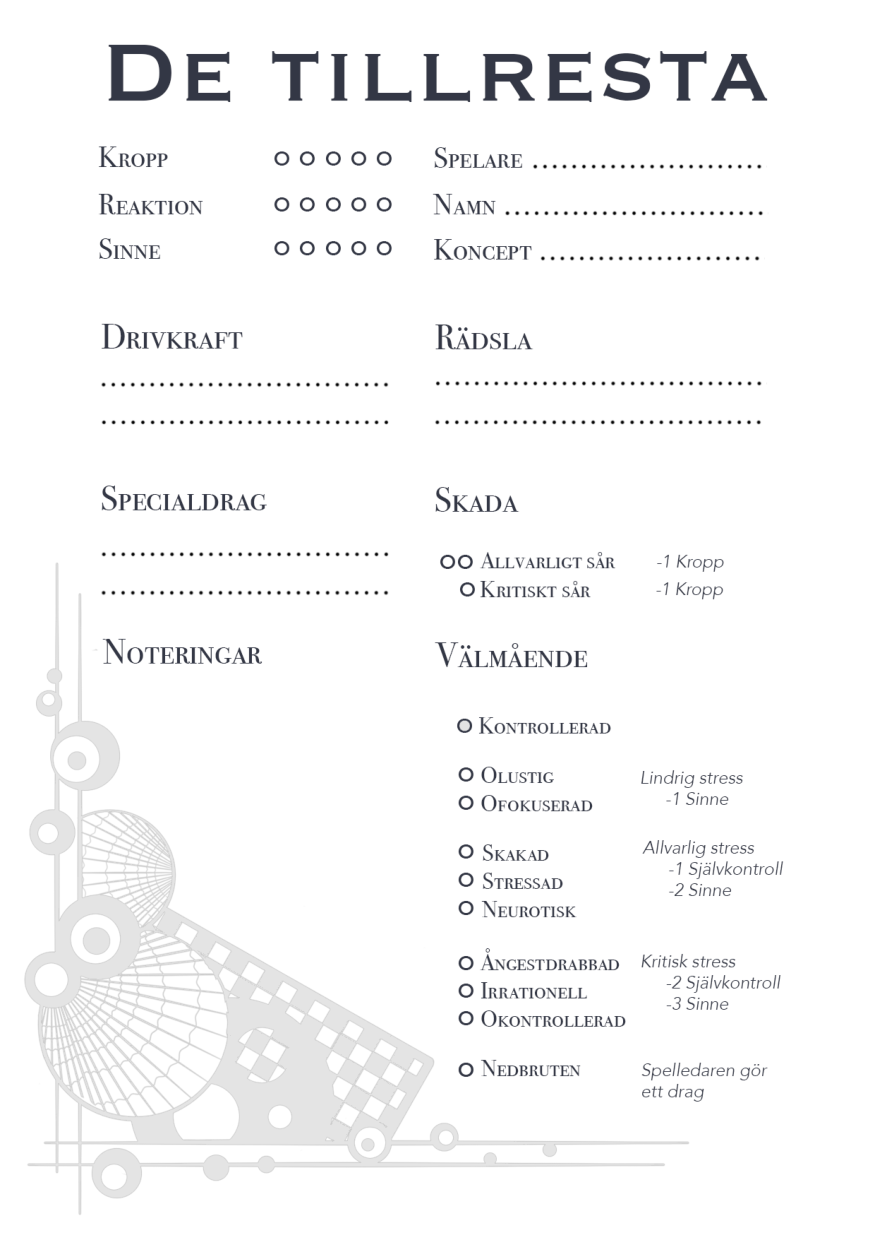
\includepdf[pages=-]{Tillresta-formular.pdf}
\end{document}
